\documentclass[a4paper,14pt]{extarticle}
\def\source{/home/osabio/tex/templates}
\input{\source/head.tex}
\yakovlev{122/123}{Электростатика}
\begin{document}

\begin{figure}[H]
    \centering
    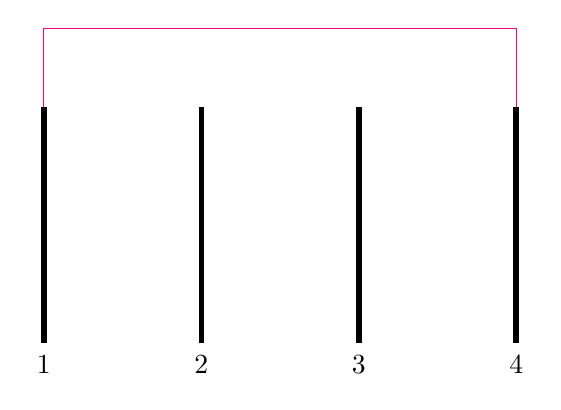
\begin{tikzpicture}
        \draw[line width=2pt] (0,0) node[below] {$1$} -- ++(0,3);
        \draw[line width=2pt] (2,0) node[below] {$2$} -- ++(0,3);
        \draw[line width=2pt] (4,0) node[below] {$3$} -- ++(0,3);
        \draw[line width=2pt] (6,0) node[below] {$4$} -- ++(0,3);

        \draw[magenta] (0,3) -- (0,4) -- (6,4) -- (6,3);      
    \end{tikzpicture} 
\end{figure}
Заменим систему эквивалентной, скомпонованной из конденсаторов:
\begin{figure}[H]
    \centering
	\begin{circuitikz}[scale=1.25, every node/.style={scale=1.25}]
		\draw (-2,0) node[anchor=east]{3}
  		to[short, o-*] (0,0)
		to[C=$C_{23}$] ++(0,2) 
		to[C=$C_{21}$] ++(2,0)
		to ++(0,-2)
		to[C=$C_{34}$] ++(-2,0);
		\draw (-2,2) node[anchor=east]{2}
  		to[short, o-*] (0,2);
	\end{circuitikz}
\end{figure}

Где $C_{34}=C_{21}$. Так как расстояние между обкладками этих конденсаторов вдвое меньше, чем у $C_{23}$, то справедливо
\begin{equation}
	C_{34}=C_{21}=2C_{23}
\end{equation}
Общая емкость конденсаторов  $C_{34}$ и $C_{21}$
\begin{equation}
	\frac{1}{C}=\frac{1}{C_{34}}+\frac{1}{C_{21}}=\frac{2}{C_{34}}
	\quad\Rightarrow\quad
	C=\frac{C_{34}}{2}=C_{23}
\end{equation}
А тогда суммарная емкость конденсаторов $C$ и $C_{23}$ будет
\begin{equation}
	C_\Sigma=C+C_{23}=2C_{23}
\end{equation}
Таким образом, емкость увеличивается вдвое. Надо учитывать, что это равенство на самом деле неточное: будут иметь место краевые эффекты, где неверны выкладки для плоского конденсатора.

\newpage
Если замкнуть одну из пластин на оболочку, то можем построить эквивалентную схему из плоских конденсаторов

\begin{figure}[H]
    \centering
	\begin{circuitikz}[scale=1.25, every node/.style={scale=1.25}]
		\draw (-2,0) node[anchor=east]{3}
  		to[short, o-*] (0,0)
		to[C=$C_{23}$] ++(0,2) 
		to[C=$C_{21}$] ++(2,0)
		to ++(0,-2)
		to[C=$C_{34}$] ++(-2,0);
		\draw (-2,2) node[anchor=east]{2}
  		to[short, o-*] (0,2);

		\draw (0,2) 
  		to[short, -*] (2,0);  		
	\end{circuitikz}
\end{figure}
Сразу понятно, что суммарная емкость будет
\begin{equation}
	C_\Sigma=C_{23}+C_{34}=C_{23}+2C_{23}=3C_{23}
\end{equation}
То есть емкость увеличится примерно втрое по сравнению с конденсатором без оболочки. Соотношение нестрогое, исходя из предыдущей оговорки.

\end{document}